\documentclass[a4paper]{article}
\newcommand{\sepspace}{\vspace*{1em}}	
%% Language and font encodings
\usepackage[english]{babel}
\usepackage[utf8x]{inputenc}
\usepackage[T1]{fontenc}

%% Sets page size and margins
\usepackage[a4paper,top=3cm,bottom=2cm,left=3cm,right=3cm,marginparwidth=1.75cm]{geometry}

%% Useful packages
\usepackage{amsmath}
\usepackage{graphicx}
\usepackage[colorinlistoftodos]{todonotes}
\usepackage[colorlinks=true, allcolors=blue]{hyperref}


\title{Ethane/air diffusion flame}

\author{Emilia Łuczak}
\date{}

\begin{document}
\maketitle
\sepspace
 \begin{centering}
 METODY KOMPUTEROWE W SPALANIU\\
 \end{centering}
 \sepspace
 \sepspace
 \sepspace
 \sepspace
 \sepspace
 \sepspace
 \sepspace
 \sepspace
 \sepspace
 \sepspace
 \sepspace
 \sepspace
 \sepspace
 \sepspace
 \sepspace
 \sepspace
 \sepspace
 \sepspace
 \sepspace
 \sepspace
 \sepspace
 \sepspace
 \sepspace
 \sepspace
 \sepspace
 \sepspace
 \sepspace
 \sepspace
 \sepspace
 \sepspace
 \sepspace
 \sepspace
 \sepspace
 \sepspace
 \sepspace
 \sepspace
 \sepspace
 \sepspace
 \sepspace
 \sepspace
 \sepspace
 \sepspace
 \sepspace
 \sepspace
 \sepspace
 
 
 \begin{centering}
 Napędy Lotnicze\\
 \end{centering}
 \begin{centering}
 Wydział Mechaniczny Energetyki i Lotnictwa\\
 \end{centering}


\pagebreak
\section{Introduction}

This paper will be dedicated to the simulation of diffusion flame. Cantera program is used to analize the temperature of an opposed-flow ethane/air diffusion flame in function of distance from burner. The temperature curves will vary depending on ambient pressure and oxidizer temperature. \\
\subsection{Input parameters}
Input parameters are as following:\\
$p = 0.25 bar$ - pressure\\
$tin_f = 300 K$ - fuel inlet temperature\\
$tin_o = 300 K$  - oxidizer inlet temperature\\
$mdot_o = 0.944 kg/m^2/s$ - stoichiometric oxidizer inlet\\
$mdot_f = 0.056 kg/m^2/s$ - stoichiometric fuel inlet \\
$comp_o = 'O2:0.21, N2:0.78, AR:0.01'$  - air composition\\
$comp_f = 'C2H6:1'$  - fuel composition\\
$width = 0.03 m$ - distance between inlets\\
\\
That means the total mixture inlet is equal to $1 kg/m^2/s$.
\\

\subsection{Analysis}
Analysis is divided into two parts. In the first one, the ambient pressure impact is examined. There are 6 variants with pressure value changing form 0.25 bar to 1.5 bar. The second part is about the impact of oxidizer initial temperature starting from 300K and ending with 700K. It is worth to notice that the oxidizer is almost 0,95 volume of the whole mixture.

\sepspace
\sepspace
\section{Mathematic model}

In order to find an equicalence ratio, following equation is needed:

\[{2C_2H_4 +7(O_2+3,76N_2) }
      = {4CO_2+6H_2 O}\] 
\\
That means there is 638.4g of oxidizer needed for 36g of fuel. It is necessarily to achieve the stoichiometric condition. Fuel-air ratio is therefore equal to $36/638.4=0.05639$.

\sepspace
\sepspace
\section{Results}
Program returns diagrams of temperature for an opposed-flow ethane/air diffusion flame in function of distance from burner with changing pressure and initial temperature in CSV format.
\pagebreak


\subsection{Ambient pressure}


All simulations were run on the assumption that the temperatures of fuel is equal to 300K and the pressure is equal to 1 bar. 

\begin{figure} [h]
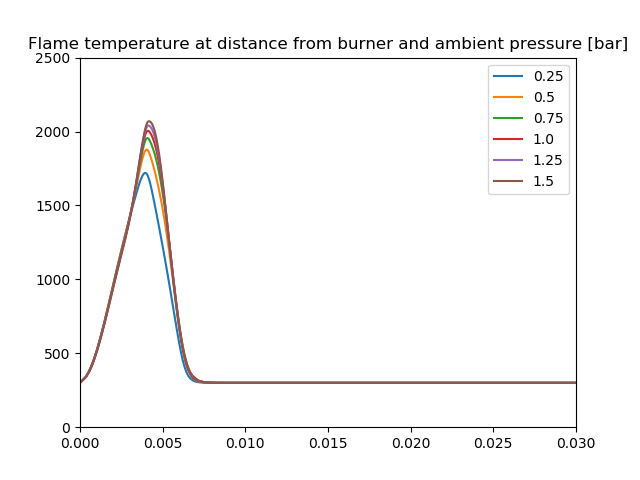
\includegraphics[width=1\textwidth]{c2h6_diffusion_pressure.png}
\caption{\label{fig:1}Temperature of an opposed-flow ethane/air diffusion flame in function of distance from burner at different pressure.}
\end{figure}

\sepspace
The temperature rapidly grows and is the highest at 0.005m distance from burner. The highest temperature is reached for the highest pressure. At about 0.007m distance the temperature is the same as the initial one, that is 300K.

\pagebreak

\subsection{Inition air temperature}
All simulations were run on the assumption that the temperatures of fuel is equal to 300K and the pressure is equal to 1 bar. 



\begin{figure}[h]
\centering
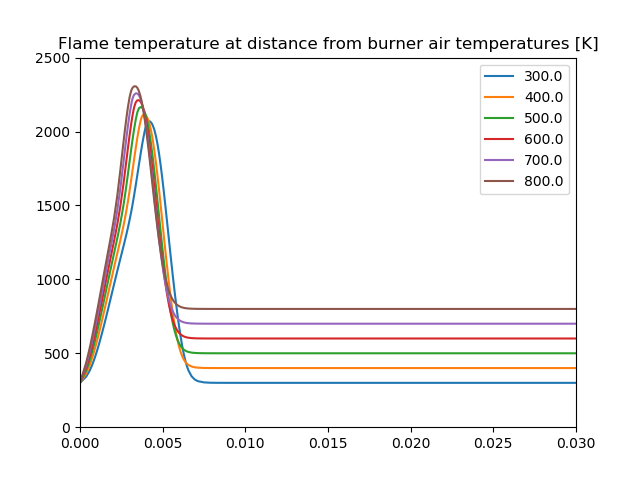
\includegraphics[width=1\textwidth]{c2h6_diffusion_temperature.png}
\caption{\label{fig:2}Temperature of an opposed-flow ethane/air diffusion flame in function of distance from burner at different oxidizer temperature.}
\end{figure}

\sepspace
The temperature rapidly grows and is the highest at 0.004m  distance form the burner for 800 K and 0.005m distance for 300K. As expected, the highest temperature is reached for the highest initial  temperature. At about 0.007m distance the temperature is the same as the initial one.

\pagebreak


\section{Conclusions}
Calculation results for different temperatures and pressures are similar to experimental results for ethanol/air diffusion flame. You can see that the characteristic of the charts is the same as in examples below. 
 


\begin{figure} [h]
\centering
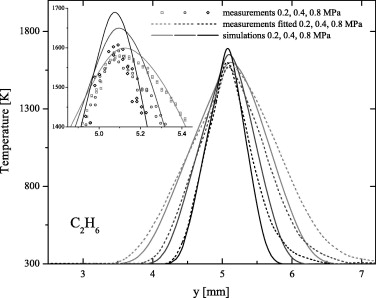
\includegraphics[width=0.7\textwidth]{01.png}
\caption{\label{fig:3}Profiles of temperature as a function of distance from the fuel boundary for ethane diffusion flames at 0.2, 0.4 and 0.8 MPa. From source [2]}
\end{figure}

bob

\begin{figure} [h]
\centering
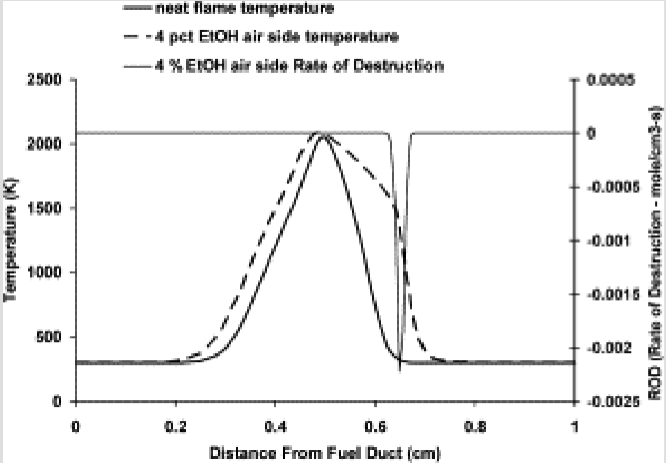
\includegraphics[width=0.7\textwidth]{02.png}
\caption{\label{fig:4}. Calculated temperature profile for air side addition of ethanol, overlaid with overall rate of destruction of ethanol vapor. From source [3]}
\end{figure}



\sepspace

\sepspace

\sepspace

\section{References}

$
\hspace{5,35mm}[1] 
www.cantera.org/examples/python/onedim/diffusion_flame.py.html
$

$
[2] www.sciencedirect.com/science/article/pii/S0010218013002897
$

$
[3] www.sciencedirect.com/science/article/pii/S001021800500115X
$

$
[4]
www.cantera.org/examples/python/onedim/diffusion_flame_batch.py.html
$


\end{document}
